\begin{frame}
    \frametitle{Příklad - JavaScript}
    \begin{figure}
        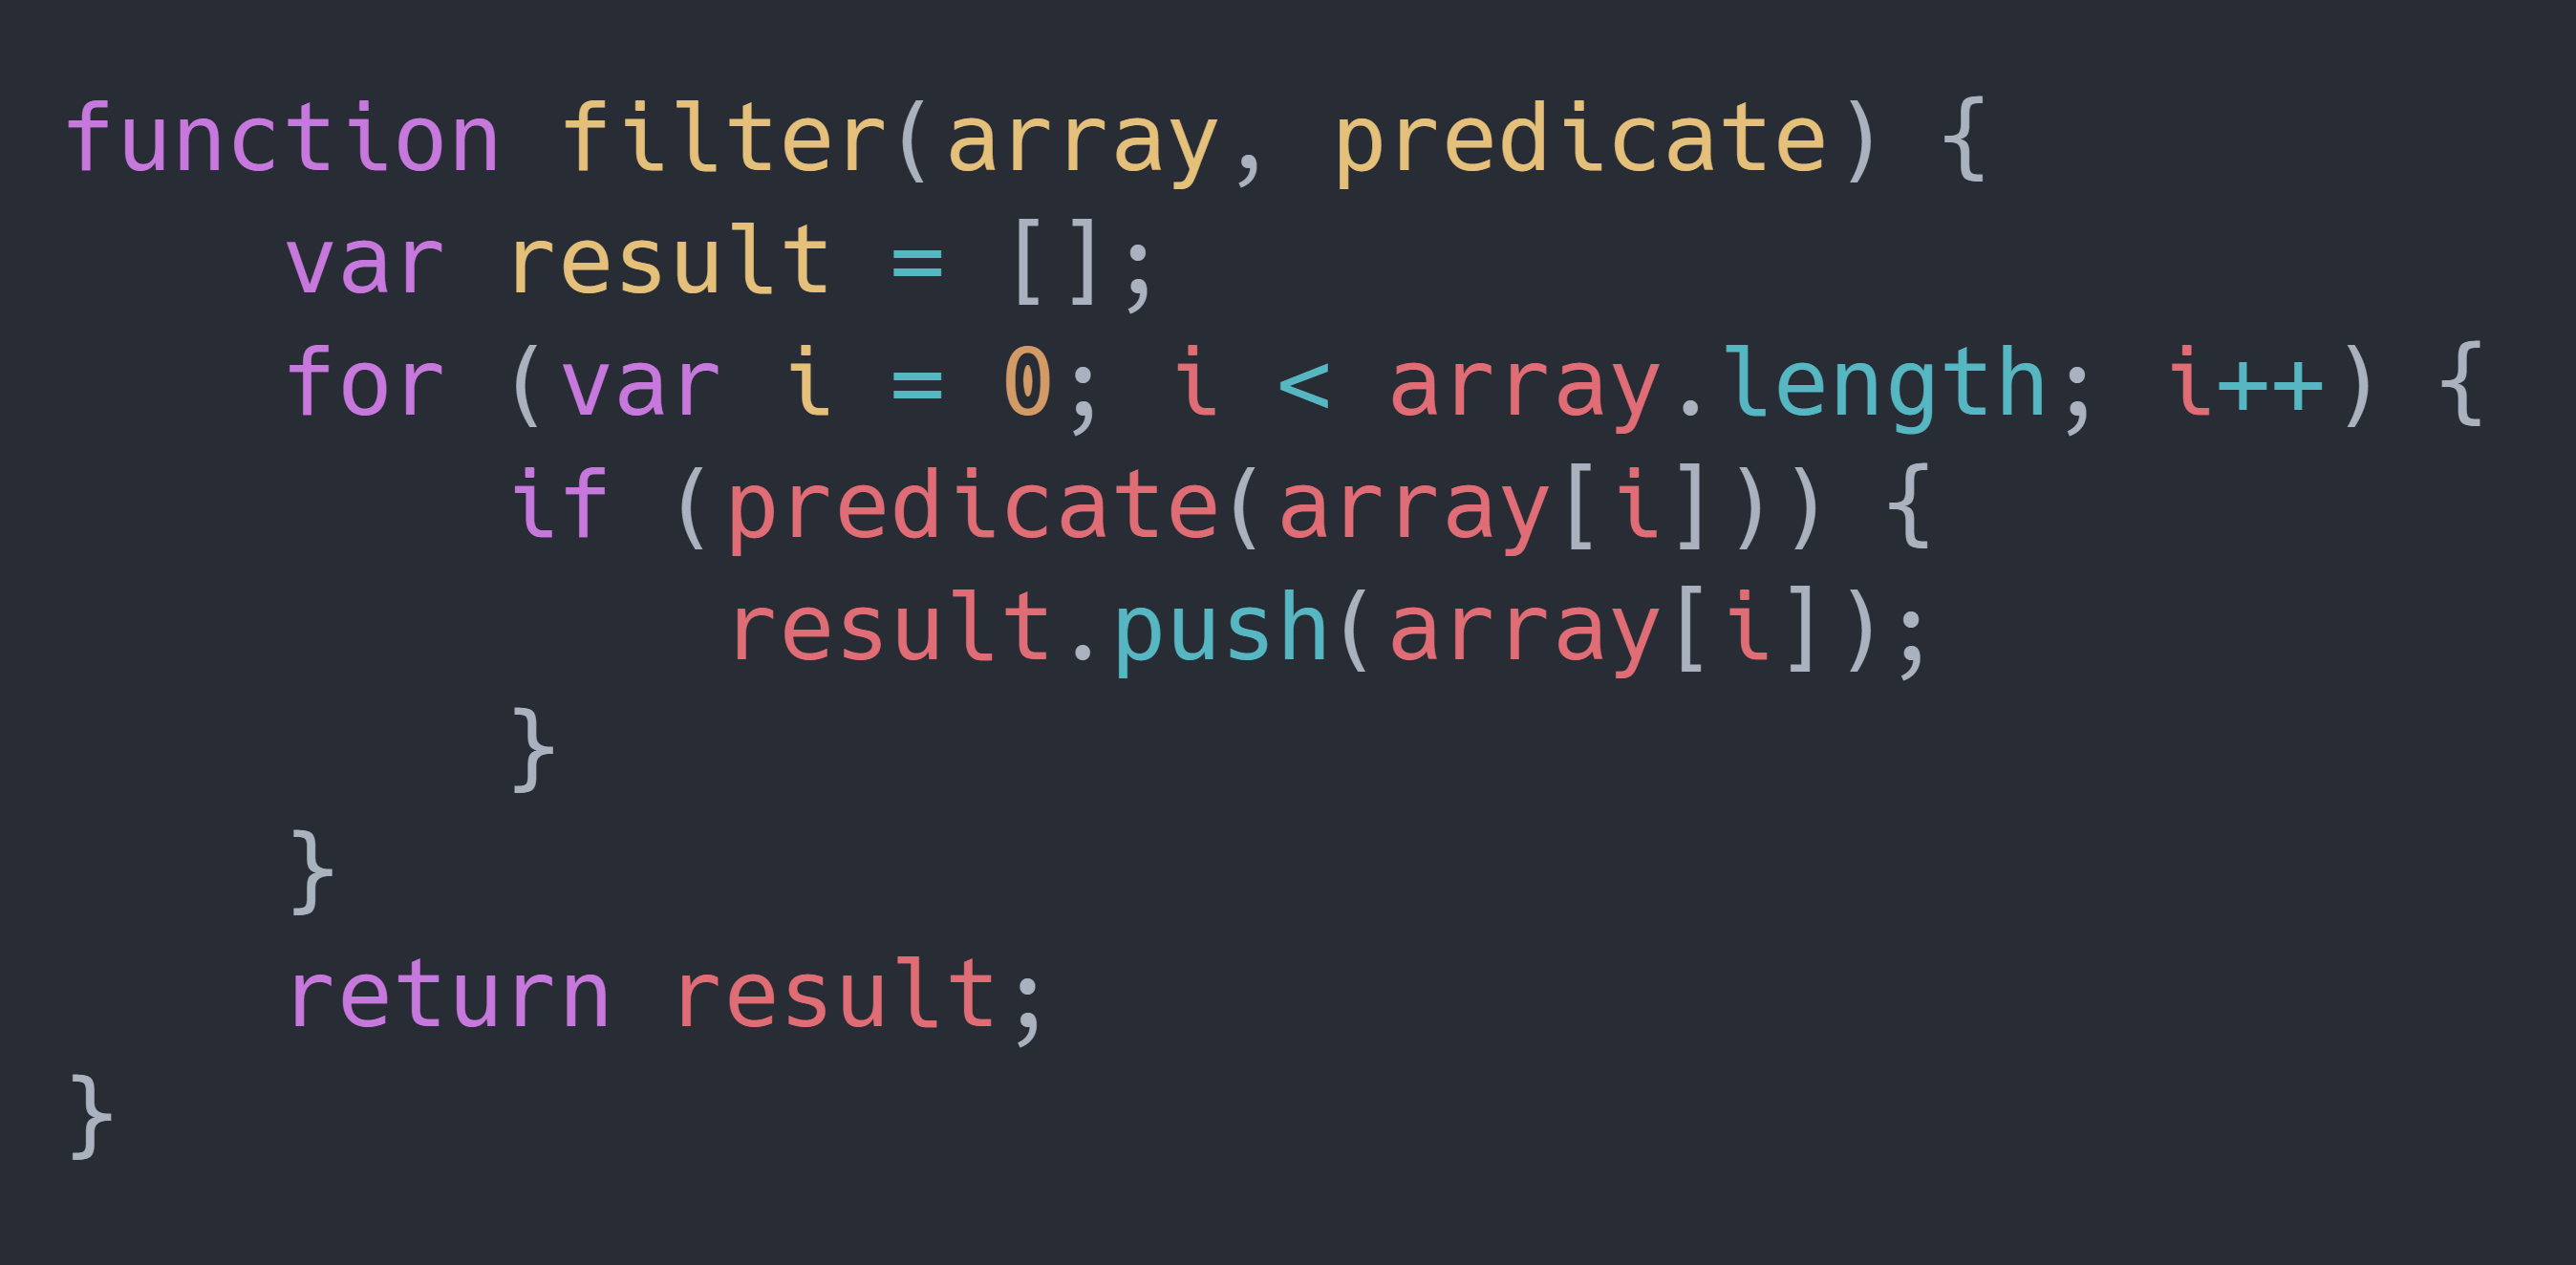
\includegraphics[width=300pt]{../resources/snippets/tsExample/example.js.png}
        \caption[Vanilla JavaScript]{Příklad implementace funkce \texttt{filter}\cite{wikipedia:filter_function} v jazyce JavaScript.}
    \end{figure}
\end{frame}

\begin{frame}
    \frametitle{Příklad - TypeScript}
    \begin{figure}
        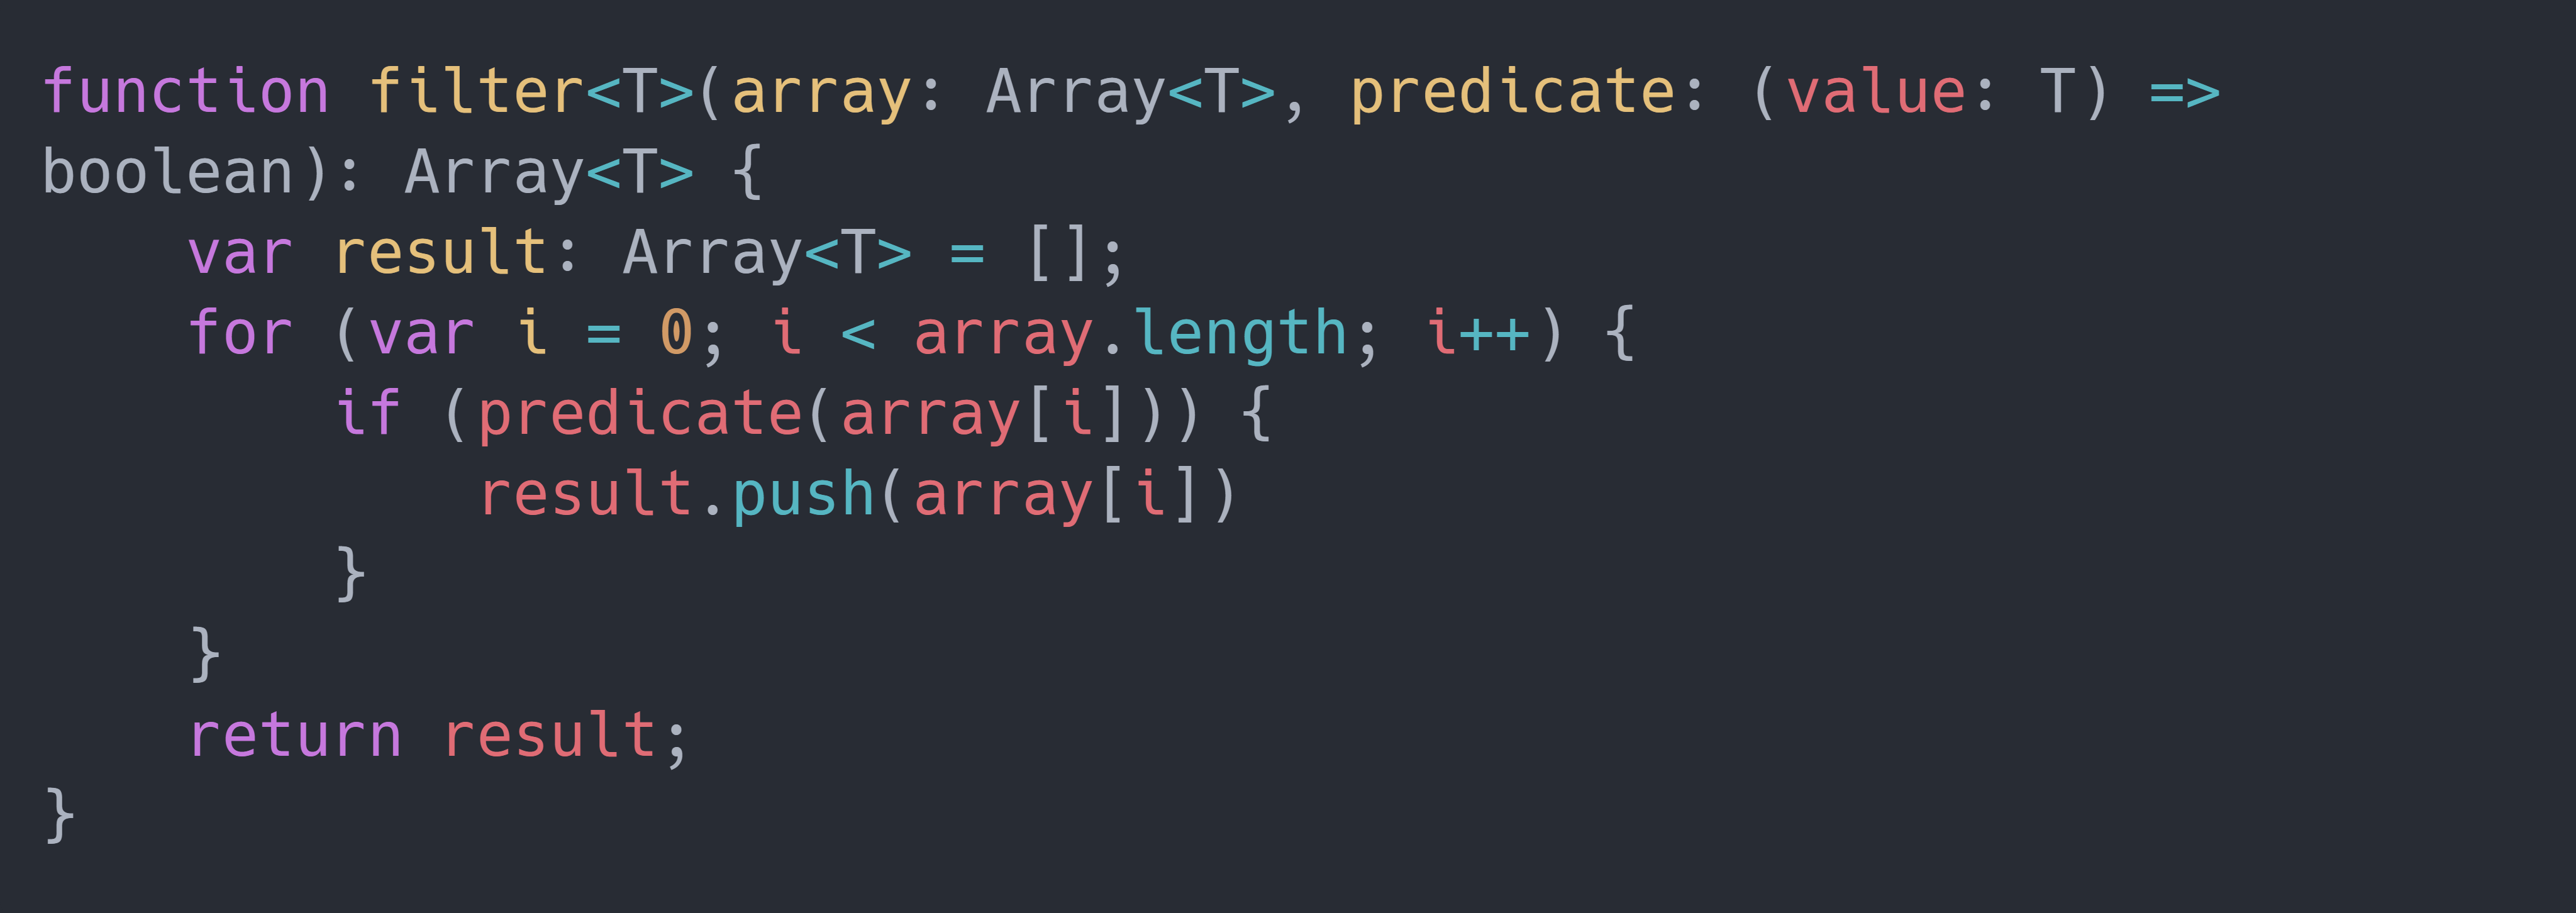
\includegraphics[width=300pt]{../resources/snippets/tsExample/example_rewritten.ts.png}
        \caption[Přepis do TypeScriptu]{Přepis funkce z předchozího slidu do TypeScriptu.}
    \end{figure}
\end{frame}

\begin{frame}
    \frametitle{Příklad - TypeScript (moderní syntaxe)}
    \begin{figure}
        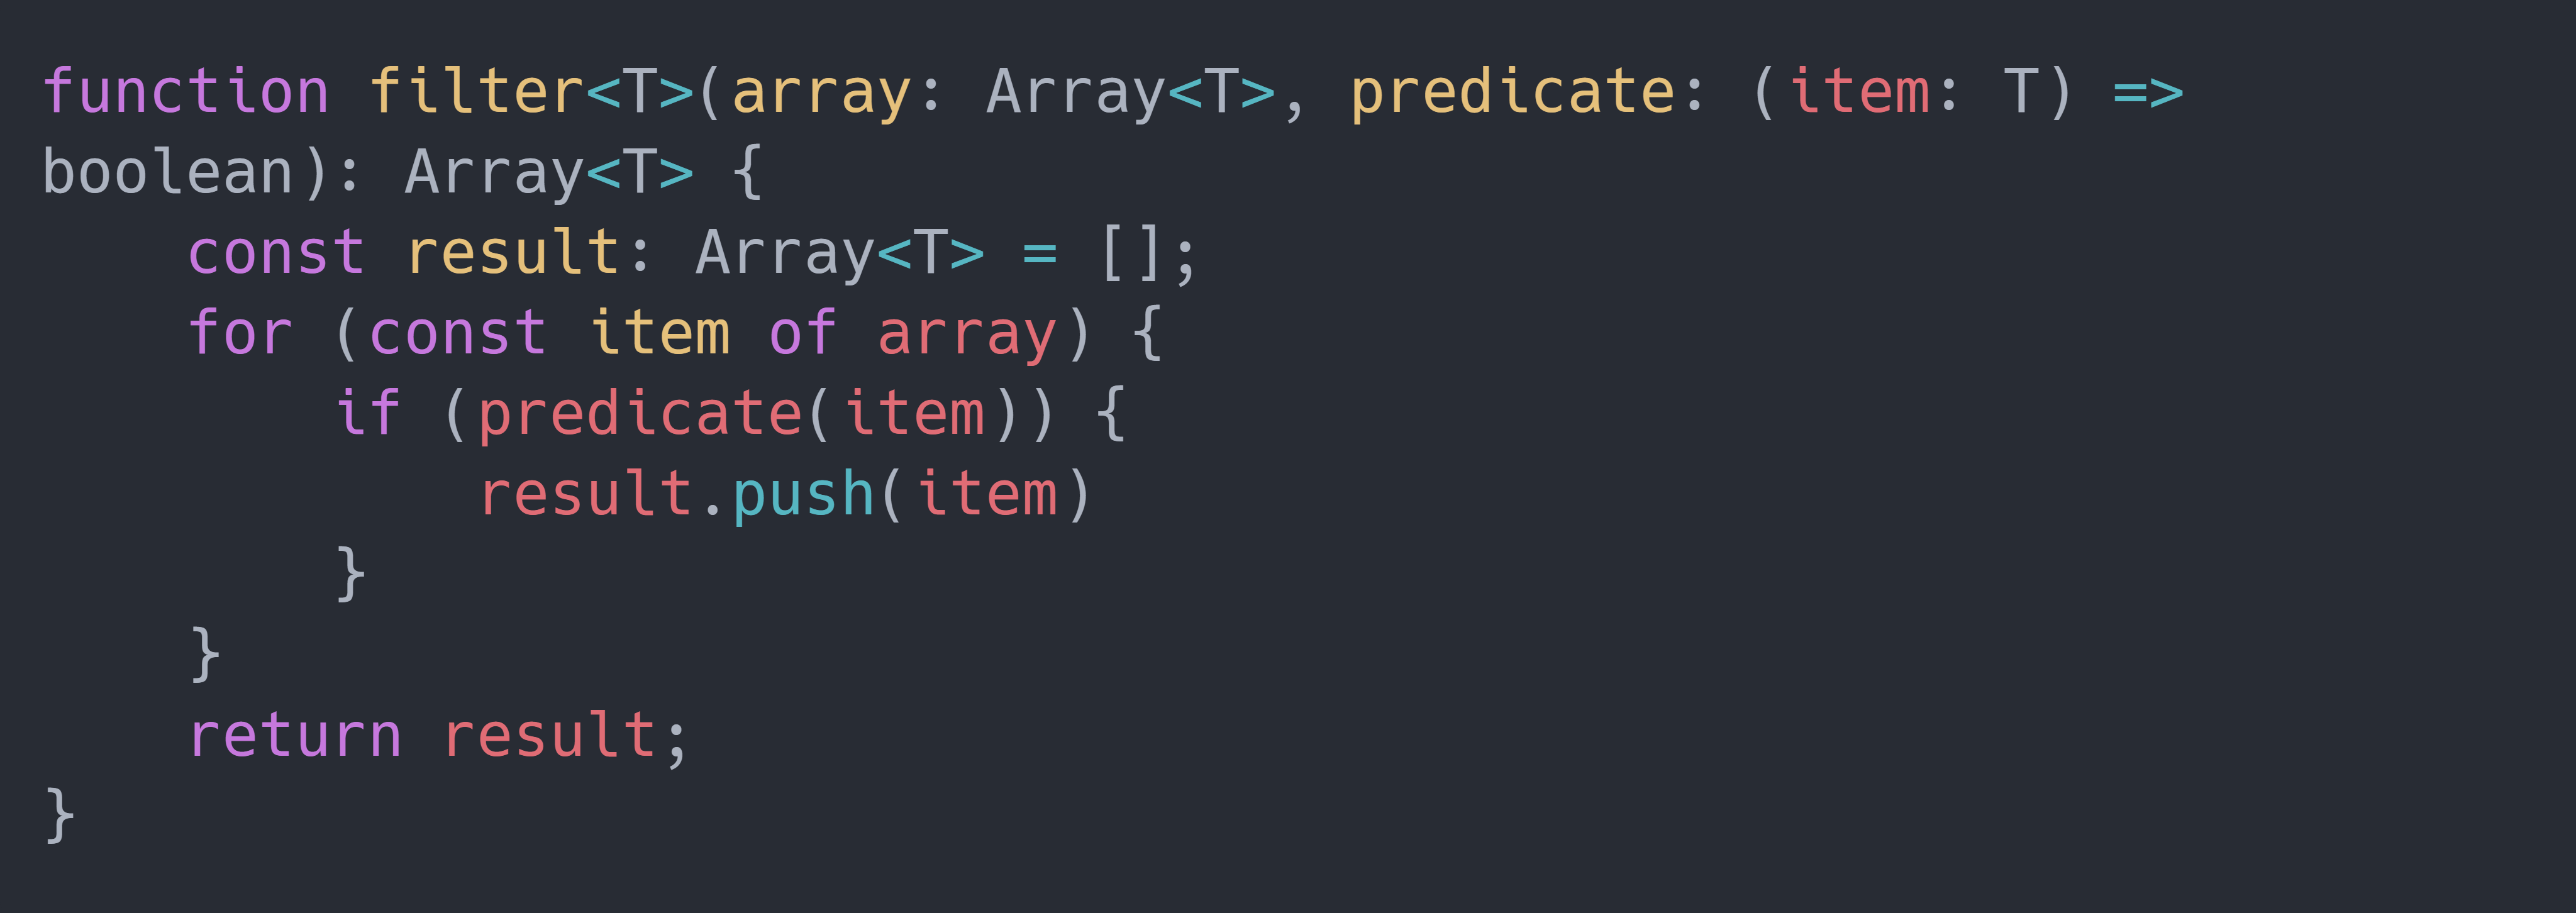
\includegraphics[width=300pt]{../resources/snippets/tsExample/example_modern.ts.png}
        \caption[TypeScript s moderní syntaxí]{Přepis funkce z předchozího slidu za použití moderní syntaxe.}
    \end{figure}
\end{frame}